% File name: documentation.tex
% Date:      13.12.2011 16:13
% Authors:   Radek Fér          <xferra00@stud.fit.vutbr.cz>
%            Miroslav Paulík    <xpauli00@stud.fit.vutbr.cz>

\documentclass[a4paper,12pt]{article}
\usepackage[czech]{babel}
\usepackage{color}
\usepackage{tabularx}
\usepackage{hyperref}
\usepackage[utf8]{inputenc}
\usepackage[left=2cm, top=3cm, text={17cm, 24cm}]{geometry}
\usepackage{graphicx} % for .eps images
\usepackage{fancyvrb,fancybox,calc}
\usepackage[svgnames]{xcolor}
\usepackage{mathtools}
 
\hypersetup{linktoc=all}
%\hypersetup{pdfborder={0 0 0 [0 0]}
\hypersetup{colorlinks=true}
\hypersetup{linkcolor=blue}

% European layout (no extra space after `.')
\frenchspacing

% no indent, free space between paragraphs
\setlength{\parindent}{0pt}
\setlength{\parskip}{1ex plus 0.5ex minus 0.2ex}

\begin{document}
\renewcommand{\refname}{Literatura}
\thispagestyle{empty}
{\LARGE \bf Laserový rezonátor a jeho stabilita}\\
\\
{\large
\begin{tabularx}{\textwidth}{l l X}
    Předmět: & Fyzikální optika (FYO), 2012/2013 & \\
    Student: & Miroslav Skácel \& Radek Fér & \\
    Email: & \texttt{\{xskace00|xferra00\}@stud.fit.vutbr.cz} & \\
Datum: & 30.\,3.\,2013 & \\
\end{tabularx}}
\begin{center}
\line(1,0){480}
\end{center}
\section{Úvod}
Nutnou součástí většiny typů laserů je rezonátor. Tuto součástku popisujeme v nasledujícím textu. V rámci optiky lze toto téma zařadit jak do kontextu geometrické, tak do kontextu vlnové optiky.
Na začátek jsme umístili kapitolu Princip laseru, kde popisujeme jevy nutné pro další pochopení. Poté už následuje hlavní část Rezonátor.

\section{Princip laseru}
Laser (zkratka pro Light Amplification by Stimulated Emission of Radiation), česky znamená zesilování světla stimulovanou emisí záření. Jak již z názvu vyplývá, klíčovým procesem k činnosti laseru je stimulovaná emise. K sestavení laseru potřebujeme 3 hlavní stavební prvky: buzení (pump), aktivní zesilující prostředí (amplifying medium) a rezonátor (resonator).

\begin{figure}[h!]
  \centering
    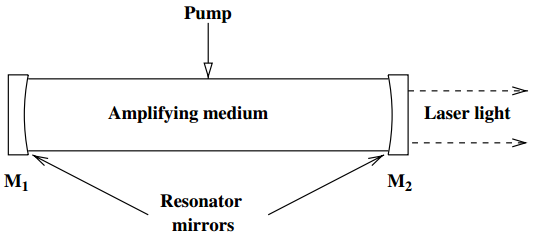
\includegraphics[width=0.5\textwidth]{images/image02.png}
    \caption{Základní stavební prvky laseru \cite{optics}}
\end{figure}

Buzení dodává laseru energii, přesněji excituje (vybudí) částice v aktivním prostředí, což je potřebné pro proces stimulované emise. Buzení je tvořeno např. výbojkou (shodnou jako ve fotoaparátech) v monokrystalyckých laserech, nebo třeba stejnosměrným elektrickým výbojem v řádu kilovoltů v plynových laserech. Aktivní prostředí laseru je složeno z materiálu, jehož částice se mohou nácházet ve více kvantových energetických vrstvách (základní a vyšší vrstvy). 
Materiály typicky požívané v laserech jsou:
\begin{itemize}
\item plyn nebo jejich směsice. Buzení prováděno opticky nebo elektricky He-Ne, CO, CO$_2$, Xe, Ar, N, H, I, Cu (výpary mědi)
\item pevná látka. Buzení opticky (laserovými diodami) - rubín, Nd:YAG, Ho:YAG, Ti-safír
\item polovodič (PN přechod) - laserová dioda (slouží pro buzení jiných typů laserů) - Ga-As, Ga-N, Ga-Al-As
    \end{itemize}

Poslední a neméně důležitou součástí laseru je optický rezonátor, který se obvykle skládá ze soustavy zrcadel a umožňuje tak opakovaný průchod fotonů aktivním zesilujícím prostředí. Bez rezonátoru by fotony opustily aktivní prostředí po prvním průchodu, čímž by nezískaly dostatek energie a navíc by se pohybovaly ve všech směrech.

\subsection{Stimulovaná emise}
Poznamenejme, že izolované částice (atom, ion, molekula) v aktivním prostředí se mohou nacházet buď ve stavu s nejnižší energií (označíme $E_0$, základní vrstva) nebo ve stavech vyšší energie $E_x$, jak bylo zmíněno dříve. Přechody mezi těmito energetickými vrstvami jsou zbůsobeny absorpcí nebo emisí.
Absorpce je proces, kdy foton o frekvenci $\nu$ narazí do částice v základní energetické vrstvě $E_0$. Tato částice se dostane do vyšší energetické vrstvy $E_x$, foton s energií $h\nu$je zcela pohlcen. Platí zde zákon o zachování energie, tedy $h\nu = E_x - E_0$.
Před vynálezem laseru byly dostupné zdroje světla založeny na spontánní emisi. Při spontánní emisi dochází k samovolnému vyzařování fotonů vybuzenými částicemi ve vyšších vrstvách. Vybuzená částice přechází samovolně z vyšší energetické hladiny $E_x$ do hladiny základní $E_0$ a přitom je vyzářen foton(elmag. vlna) o frekvenci $\nu = (E_x-E_0)/h$. Fotony jsou vyzařovány v náhodném směru, s různou fází a polarizací. Záření vznikající při spontánní emisi je tedy nekoherentní. Emise se jmenuje spontánní proto, že není spouštěna žádným vnějším vlivem, ale vzniká samovolně. Na tomto principu funguje např. klasická žárovka.
Střední doba života setrvání částice (lifetime) ve vyšší energetické vrstvě $E_x$ je řádově $10^{-8}s$ (short lifetime). To je pro činnost laseru nedostačující. Proto se používají materiály s více energetickými vrstvami, kde se excitovaná částice dostane pomocí spontanní emise do nižší (ne však základní) energ. vrstvy, přičemž nedochází k vyzáření fotonu. V této vrstvě může pak setrvat až $10^{5}\times$ déle (long lifetime). Tento stav se nezývá metastabilní a je nezbytný pro správnou činnost laseru.

Další důležitý pojem je inverze populace. K inverzi populace dochází v situaci, kdy je více excitovaných částic v metastabilním vrstvě než ve vrstvě základní, platí tedy $n_2 > n_1$, kde $n_x$ je počet částic (populace) v energ. vrstvě $x$.
V laserech se využívá stimulované emise (vynucená emise). Při stimulované emisi dopadá foton o frekvenci $\nu$ na částici ve vyšší energetické vrstvě $E_x$ a tím ho přiměje k přechodu do základní energetické vrstvy $E_0$, dojde k vyzáření fotonu se stejnou frekvencí, fází, polaritou a směru šíření jako dopadající foton. Tento původní foton ale není pohlcen (absorbován částicí), takže dojde k jeho složení s vyzářeným fotonem. Opět zde platí zákon o zachování energie, platí $h\nu + A(E_x) \rightarrow A(E_0) + xh\nu$, kde $A(E)$ značí částici $A$ v energ. stavu $E$. Záření vznikajcí při stimulované emisi je koherentní. Stimulovanou emisí při inverzi populace (vetšina částic je v excitovaném stavu) lze spustit řetězovou reakci stimulujících procesů jediným fotonem o správné frekvenci $\nu$.
Na tomto principu je tvořen laserový paprsek.

\begin{figure}[h!]
  \centering
    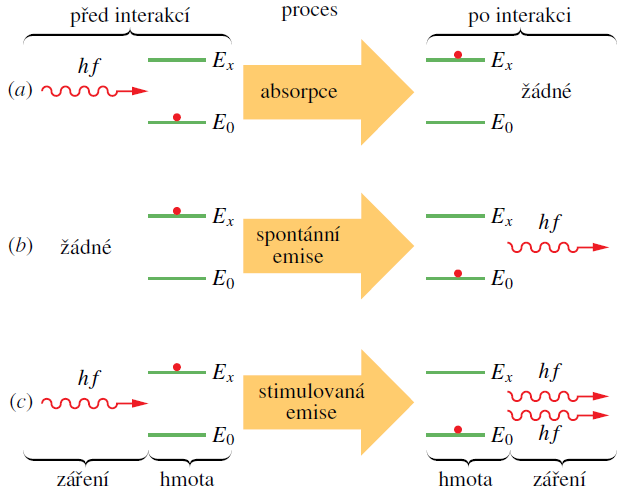
\includegraphics[width=0.5\textwidth]{images/image05.png}
    \caption{Absorpce, spontánní a stimulovaná emise \cite{hrw}}
\end{figure}


\begin{figure}[h!]
  \centering
    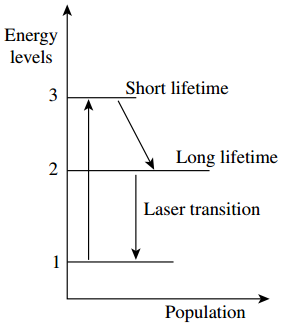
\includegraphics[width=0.25\textwidth]{images/image01.png}
\caption{Metastabilní stav excitovaných částic (3-vrstvý) \cite{optics}}
\end{figure}


\section{Rezonátor}
U většiny typů laserů je nutné pro zvýšení poměru emise stimulované ku spontánní dosáhnout dostatečné hustoty energie (incidentních fotonů) pomocí tzv. rezonátoru.
Jde o soustavu zrcadel namířených proti sobě, která jsou od sebe vhodně vzdálena.
Účinnost těchto zrcadel musí být většinou velmi vysoká (\textgreater 95\%), podle toho, jakou vlnovou délku laser produkuje. Obecně se dá říci, že čím kratší vlnová délka, tím vyšší hustoty energie musí rezonátor dosáhnout. \cite{funds}. To je také důvod, proč dříve než lasery existovaly masery.
Fotony (elmag. vlny, chcete-li) mezi těmito zrcadly oscilují a část z nich uniká ve formě laserového svazku jedním ze zrcadel, které je polopropustné. Pro správnou funkci rezonátoru musí být splněny následující podmínky:
\begin{itemize}
\item Emitované fotony nejsou zcela pohlceny zpět prostředím. Tedy musí platit $\frac{r_{stimulated}}{r_{absorption}} = \frac{N_2}{N_1}$. Pokud jsme ale dosáhli v médiu inverze populace, platí $N_2>N_1$, a tedy platí i tato podmínka.
\item Vzdálenost zrcadel je $q\frac{\lambda}{2}$, kde $q$ je tzv. mód rezonátoru a $\lambda$ je vlnová délka světla laseru. Tato podmínka zaručuje konstruktivní interferenci kolidujících paprsků (stojaté vlnění).
\item Optická soustava je stabilní. Tzn. paprsky světla jsou i po několika odrazech stále v zajetí rezonátoru. Při porušení této podmínky se fotony po několika odrazech dostávají z prostoru rezonátoru a energie z rezonátoru tak zbytečně uniká.

\end{itemize}

\begin{figure}[h!]
  \centering
  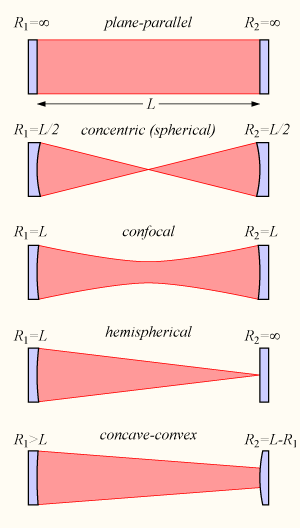
\includegraphics[width=0.25\textwidth]{images/image00.png}
\caption{Základní konfigurace laserových rezonátorů ($R_1$ a $R_2$ jsou poloměry zrcadel, $L$ je vzdálenost těchto zrcadel) \cite{cavity}.}
\end{figure}

\section{Stabilita}
Laserové rezonátory se používají v několika různých konfiguracích, proto je nutné stanovit definici stability rezonátoru. Stabilita je chápána jako schopnost stálého udržení paprsků uvnitř optické soustavy. Každý paprsek se po průchodu rezonátorem odrazí od zrcadel a musí se vrátit do původního směru, ve kterém se pohyboval v předchozím průchodu. Ke splnění této podmínky je potřeba nastavit konfiguraci rezonátoru takovou, kdy je paprsek zcela zachycen uvnitř soustavy. Každé ze zrcadel popíšeme parametrem $g$, platí vztah $g=1-\frac{L}{r}$, kde $L$ je vzdálenost zrcadel a $r$ je poloměr zrcadla. Stabilita je pak definována vztahem $0 \leq g_1g_2 \leq 1$, kde $g_1$ a $g_2$ jsou parametry obou zrcadel. V případě planparalelní konfigurace rezonátoru, kdy $r_1 = r_2 = \infty$, pak $g_1 = g_2 = 1$ a stabilita tedy dosahuje hodnoty 1.
V případě konfokální konfigurace je $r_1 = r_2 = L$, pak $g_1 = g_2 = 0$ a stabilita má hodnotu 0.
Stabilitu optické soustavy lze zobrazit grafem, kde jednotlivé osy znázorňují $g$ parametry obou zrcadel.



\begin{figure}[h!]
  \centering
    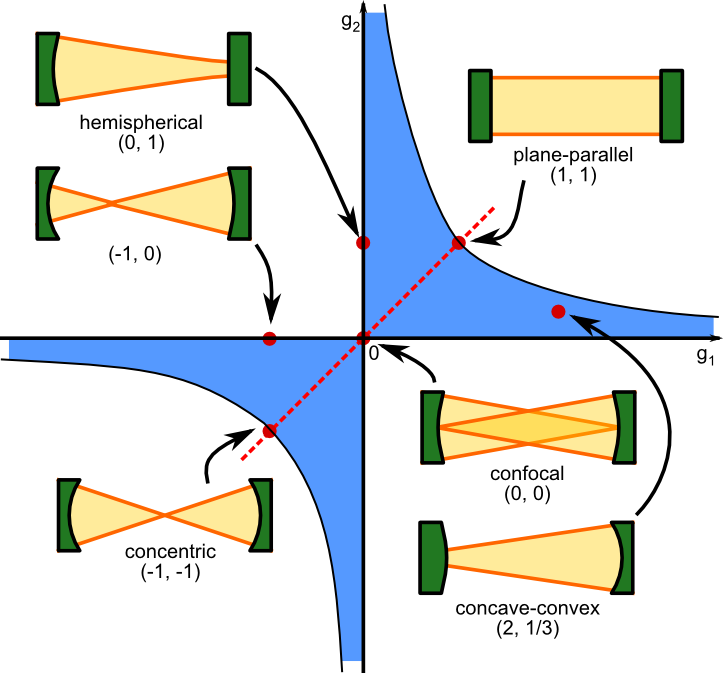
\includegraphics[width=0.5\textwidth]{images/image03.png}
\caption{Graf stability pro rezonátor se dvěma zrcadly. Konfigurace v modré oblasti jsou stabilní \cite{cavity}}
\end{figure}


\section{Ovození podmínky stability}


\begin{figure}[h!]
  \centering
    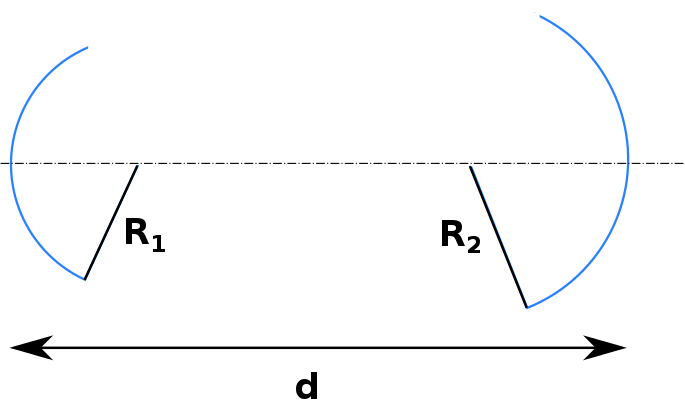
\includegraphics[width=0.5\textwidth]{images/image04.png}
\caption{Schématický nákres rezonátoru vytvořeného ze dvou sférických zrcadel.}
\end{figure}

Na obrázku 6 vidíme rezonátor tvořený dvěma sférickými zrcadly o poloměrech $R_1$ resp. $R_2$. Vzdálenost mezi těmito zrcadly je $d$. Pro stabilní rezonátory musí platit, že paprsek je i po několika odrazech směrován stále na protější zrcadlo.

Uvažujme nyní pouze cestu jednoho paprsku rezonátorem. Paprsek začne svou cestu u prvního zrcadla, urazí vzdálenost $d$ k druhému zrcadlu od nějž se odrazí, znovu urazí vzdálenost $d$ a odrazí se od prvního zrcadla. S využitím znalostí z maticové optiky toto můžeme zapsat jako sled charakteristických matic pro cestu paprsku homogenním prostředím a pro odraz na kulovém zrcadle:
$$
S = R_1T_dR_2T_d = 
\begin{pmatrix}
1 & 0 \\
\frac{2}{R_1} & 1
\end{pmatrix}\begin{pmatrix}
1 & d \\
0 & 1
\end{pmatrix}\begin{pmatrix}
1 & 0 \\
\frac{2}{R_2} & 1
\end{pmatrix}\begin{pmatrix}
1 & d \\
0 & 1
\end{pmatrix} = \begin{pmatrix}
A & B\\
C & D
\end{pmatrix},$$ kde
$$
A=1+\frac{2d}{R_2},
B=2d(1+\frac{d}{R_2}),
C=2(\frac{1}{R_1} + \frac{1}{R_2}(1+\frac{2d}{R_1})),
D=\frac{2d}{R_1} + (1 + \frac{2d}{R_1})(1+\frac{2d}{R_2}).
$$
Tedy můžeme psát:
$$
\begin{pmatrix}
x_1 \\
\nu_1
\end{pmatrix} = \begin{pmatrix}
A & B\\
C & D
\end{pmatrix}\begin{pmatrix}
x_0 \\
\nu_0
\end{pmatrix}
$$

Dvojice $(x_1, \nu_1)$ jsou tedy nové parametry paprsku po jednom průchodu rezonátorem. Po $m$ průchodech budou mít nové paprsky parametry
$$
\begin{pmatrix}
x_m \\
\nu_m
\end{pmatrix} = \begin{pmatrix}
A & B\\
C & D
\end{pmatrix}^m\begin{pmatrix}
x_0 \\
\nu_0
\end{pmatrix}
$$

Lze ukázat \cite{eowm}, že
$$
\begin{pmatrix}
A & B\\
C & D
\end{pmatrix}^m = \frac{1}{\sin \theta}\begin{pmatrix}
A \sin(m\theta) - \sin((m-1)\theta) & B \sin(m\theta) \\
C \sin(m\theta) & D \sin((m-1)\theta)
\end{pmatrix},
$$

kde úhel $\theta$ je definován jako $\cos\theta = \frac{1}{2}(A+D)$.

Pro stabilní rezonátor by neměly souřadnice paprsku divergovat pro $m \rightarrow \infty$. To se nestane, pokud bude velikost $\cos\theta$ menší než 1. Jinými slovy, pokud je $\theta$ komplexní číslo, výrazy $\sin(m \theta)$ a $\sin((m-1)\theta)$ divergují. Odtud je tedy podmínka pro stabilitu následující:
$$
-1 \le \cos\theta \le 1
$$
nebo ekvivalentně (po úravách z předchozích rovnic):
$$
0 \le (1+\frac{d}{R_1})(1+\frac{d}{R_2}) \le 1.
$$

\bibliographystyle{plain}
\bibliography{literatura}
\end{document}
